\documentclass[landscape]{article}
\usepackage[margin=0.4in]{geometry}
\usepackage{tikz}
\usepackage{amsmath}
\usepackage{amssymb}
\usepackage{graphicx}
\usetikzlibrary{arrows.meta, positioning, calc}

\makeatletter
\newcommand{\fontsubtiny}{\@setsize\fontsubtiny{5pt}\ivpt\@vpt}
\makeatother

\begin{document}
\thispagestyle{empty}

\begin{center}
\resizebox{\textwidth}{!}{%
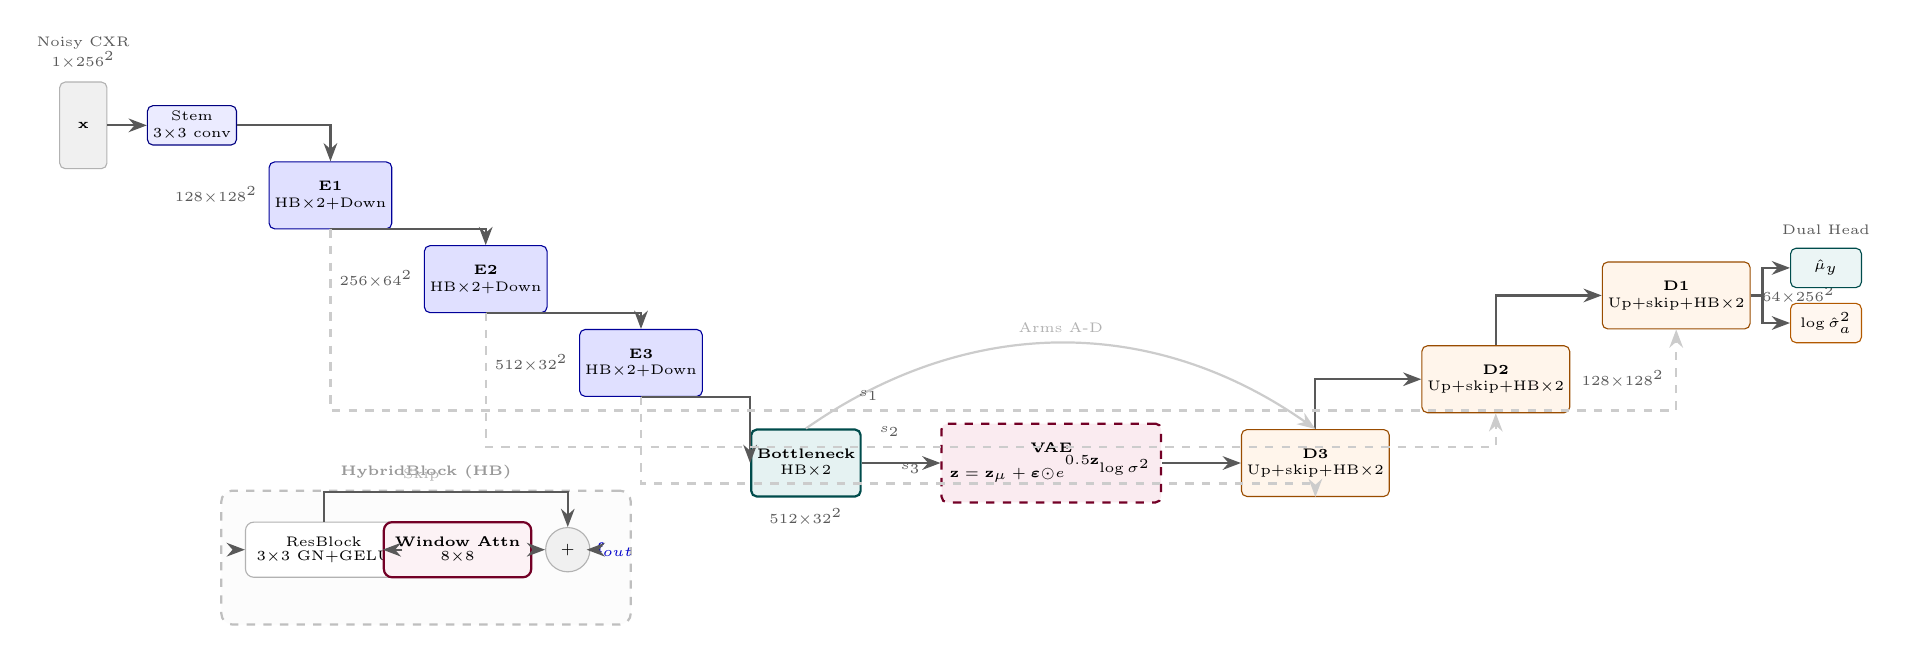
\begin{tikzpicture}[
  >=Stealth,
  node distance=0.4cm and 0.5cm,
  every node/.style={font=\tiny},
  imgnode/.style={draw=gray!60, fill=gray!12, rounded corners=2pt, minimum width=0.6cm, minimum height=1.1cm, align=center, inner sep=2pt},
  stemnode/.style={draw=blue!50!black, fill=blue!8, rounded corners=2pt, minimum width=0.8cm, minimum height=0.5cm, align=center, inner sep=2pt},
  encnode/.style={draw=blue!60!black, fill=blue!12, rounded corners=2pt, minimum width=0.9cm, minimum height=0.85cm, align=center, inner sep=2pt},
  botnode/.style={draw=teal!60!black, fill=teal!10, rounded corners=2pt, minimum width=1.3cm, minimum height=0.85cm, align=center, inner sep=2pt, thick},
  vaenode/.style={draw=purple!60!black, fill=purple!8, rounded corners=2pt, minimum width=2.2cm, minimum height=1.0cm, align=center, inner sep=3pt, dashed, thick},
  decnode/.style={draw=orange!60!black, fill=orange!8, rounded corners=2pt, minimum width=0.9cm, minimum height=0.85cm, align=center, inner sep=2pt},
  outnode/.style={draw=teal!60!black, fill=teal!8, rounded corners=2pt, minimum width=0.9cm, minimum height=0.5cm, align=center, inner sep=2pt},
  hbbox/.style={draw=gray!50, fill=gray!2, dashed, rounded corners=4pt, thick},
  insetnode/.style={draw=gray!60, fill=white, rounded corners=3pt, align=center, inner sep=4pt, font=\fontsubtiny},
  wa_style/.style={draw=purple!60!black, fill=purple!5, rounded corners=3pt, align=center, inner sep=4pt, font=\fontsubtiny, thick},
  add_style/.style={draw=gray!60, fill=gray!12, circle, minimum size=0.4cm, align=center, font=\fontsubtiny},
  dimtag/.style={font=\fontsubtiny, text=gray!70!black, align=center},
  inset_dimtag/.style={font=\fontsubtiny\bfseries, text=blue!80!black},
  arrmain/.style={->, thick, gray!70!black},
  arrskip/.style={->, gray!40, dashed, thick},
  arrvae/.style={->, purple!70!black}
]

  % ════════════════════════════════════════════════════════════════
  % ENCODER PATH
  % ════════════════════════════════════════════════════════════════
  
  \node[imgnode] (inp) {$\mathbf{x}$};
  \node[above=0.04cm of inp, dimtag] {Noisy CXR\\$1{\times}256^{2}$};

  \node[stemnode, right=of inp] (stem) {Stem\\{\fontsubtiny $3{\times}3$ conv}};

  \node[encnode, below right=0.2cm and 0.4cm of stem] (enc1) {\textbf{E1}\\{\fontsubtiny HB$\times$2+Down}};
  \node[left=0.02cm of enc1, dimtag] {$128{\times}128^{2}$};

  \node[encnode, below right=0.2cm and 0.4cm of enc1] (enc2) {\textbf{E2}\\{\fontsubtiny HB$\times$2+Down}};
  \node[left=0.02cm of enc2, dimtag] {$256{\times}64^{2}$};

  \node[encnode, below right=0.2cm and 0.4cm of enc2] (enc3) {\textbf{E3}\\{\fontsubtiny HB$\times$2+Down}};
  \node[left=0.02cm of enc3, dimtag] {$512{\times}32^{2}$};

  % ════════════════════════════════════════════════════════════════
  % BOTTLENECK, VAE, AND DECODER START
  % ════════════════════════════════════════════════════════════════
  
  \node[botnode, below right=0.4cm and 0.6cm of enc3] (bot) {\textbf{Bottleneck}\\{\fontsubtiny HB$\times$2}};
  \node[below=0.02cm of bot, dimtag] {$512{\times}32^{2}$};

  \node[vaenode, right=1.0cm of bot] (vae) {
    \textbf{VAE}\\
    {\fontsubtiny $\mathbf{z} = \mathbf{z}_\mu + \boldsymbol{\varepsilon}{\odot}e^{0.5\mathbf{z}_{\log\sigma^2}}$}
  };

  \node[decnode, right=1.0cm of vae] (dec3) {\textbf{D3}\\{\fontsubtiny Up+skip+HB$\times$2}};

  % ════════════════════════════════════════════════════════════════
  % DECODER PATH
  % ════════════════════════════════════════════════════════════════

  \node[decnode, above right=0.2cm and 0.4cm of dec3] (dec2) {\textbf{D2}\\{\fontsubtiny Up+skip+HB$\times$2}};
  \node[right=0.02cm of dec2, dimtag] {$128{\times}128^{2}$};

  \node[decnode, above right=0.2cm and 0.4cm of dec2] (dec1) {\textbf{D1}\\{\fontsubtiny Up+skip+HB$\times$2}};
  \node[right=0.02cm of dec1, dimtag] {$64{\times}256^{2}$};

  \node[outnode, right=0.5cm of dec1, yshift=0.35cm] (outmu) {$\hat{\mu}_y$};
  \node[outnode, draw=orange!70!black, fill=orange!6, right=0.5cm of dec1, yshift=-0.35cm] (outsig) {$\log\hat{\sigma}^2_a$};
  \node[above=0.04cm of outmu, dimtag] {Dual Head};

  % ════════════════════════════════════════════════════════════════
  % ROUTING ARROWS
  % ════════════════════════════════════════════════════════════════

  \draw[arrmain] (inp.east) -- (stem.west);
  \draw[arrmain] (stem.east) -| (enc1.north);
  \draw[arrmain] (enc1.south) -| (enc2.north);
  \draw[arrmain] (enc2.south) -| (enc3.north);
  \draw[arrmain] (enc3.south) -| (bot.west);
  
  \draw[arrmain] (bot.east) -- (vae.west);
  \draw[arrmain] (vae.east) -- (dec3.west);
  
  \draw[arrmain] (dec3.north) |- (dec2.west);
  \draw[arrmain] (dec2.north) |- (dec1.west);
  \draw[arrmain] (dec1.east) -- ++(0.15,0) |- (outmu.west);
  \draw[arrmain] (dec1.east) -- ++(0.15,0) |- (outsig.west);

  % Bypass path
  \draw[arrmain, gray!40, bend left=35]
    (bot.north) to node[above, font=\fontsubtiny, text=gray!60, midway, sloped] {Arms A-D} (dec3.north);

  % Rerouted skip links below the entire network to eliminate intersecting boxes
  \draw[arrskip] (enc1.south) -- ++(0,-2.3) -| node[pos=0.2, dimtag, above] {$s_1$} (dec1.south);
  \draw[arrskip] (enc2.south) -- ++(0,-1.7) -| node[pos=0.2, dimtag, above] {$s_2$} (dec2.south);
  \draw[arrskip] (enc3.south) -- ++(0,-1.1) -| node[pos=0.2, dimtag, above] {$s_3$} (dec3.south);

  % ════════════════════════════════════════════════════════════════
  % HYBRIDBLOCK DETAILS (Shifted down slightly to leave space for skip s1)
  % ════════════════════════════════════════════════════════════════
  
  \begin{scope}[shift={($(enc1.west) + (0.0, -4.5)$)}]
    \node[hbbox, minimum width=5.2cm, minimum height=1.7cm] (hbframe) at (2.0, -0.1) {};
    \node[above=0.01cm of hbframe, font=\fontsubtiny\bfseries, text=gray!80] {HybridBlock (HB)};

    \node[inset_dimtag] (fin) at (-0.1, 0) {$\mathbf{f}_{in}$};
    
    \node[insetnode, minimum width=1.5cm, minimum height=0.7cm] (rb) at (0.7, 0) {ResBlock\\3$\times$3 GN+GELU};
    \node[wa_style, minimum width=1.5cm, minimum height=0.7cm] (wa) at (2.4, 0) {\textbf{Window Attn}\\8$\times$8};
    
    \node[add_style] (add) at (3.8, 0) {$+$};
    \node[inset_dimtag] (fout) at (4.4, 0) {$\mathbf{f}_{out}$};

    \draw[arrmain] (fin) -- (rb.west);
    \draw[arrmain] (rb.east) -- (wa.west);
    \draw[arrmain] (wa.east) -- (add.west);
    
    \draw[arrmain] (rb.north) -- ++(0,0.38) -| node[pos=0.2, above, font=\fontsubtiny, text=gray!60] {Skip} (add.north);
    \draw[arrmain] (add.east) -- (fout);
  \end{scope}

\end{tikzpicture}%
}
\end{center}

\end{document}